
\section{Failure Detection Benchmarks}

The purpose of this benchmarks is to find the following four types of failures,
    \begin{itemize}
        \item Node Failure
        \item Channel Link Failure
        \item Provenance Daemon Failure
        \item Pipeline Daemon Failure
    \end{itemize}

\subsection{Node Failure}

The purpose of this benchmark is to find the time taken to detect a node failure in the topology. Node failure is here meant to be the nodes that run the provenance daemon and pipeline daemon and not the sensors. If any of the nodes that are running the provenance API daemon and pipeline daemon are failed then messages sent via this nodes will be failed to reach the other nodes.

We need to measure the time taken metric for our provenance system to detect such a node failure. In our provenance database, heartbeat messages are sent by each node are stored in the HEARTBEAT table.

So the main tables that are needed to perform this benchmark are,
    \begin{itemize}
        \item Node
        \item HeartBeat
    \end{itemize}

\subsubsection{Method to generate a node failure}

Method to simulate a node failure is to kill the container(node) itself. Here the workload generator will introduce failures continuously at regular intervals by killing the docker container and restarting the docker container. This killing and restarting process will happen throughout the benchmark.

\subsubsection{Logic used to detect node failure}

We will be querying the Node table to get the list of nodes. Once we got the node id for a particular node, then we query the heartbeat table to get the rows with that id.

Once we get the rows, if heartbeat rows are available for the node then we can be sure that the node is active. We also need to perform an additional check to find out if the timestamp field is less than 30 seconds old. Because each node will be sending the heartbeat messages every 30 seconds and we need to be sure that the node is active currently. We will store the timestamp value each time in the benchmark and compare it next time with the previous value to find out if the heartbeat message is the latest one.

\subsubsection{Result}

Following graph has been generated from the results obtained,

\begin{figure}[H]
	\center
	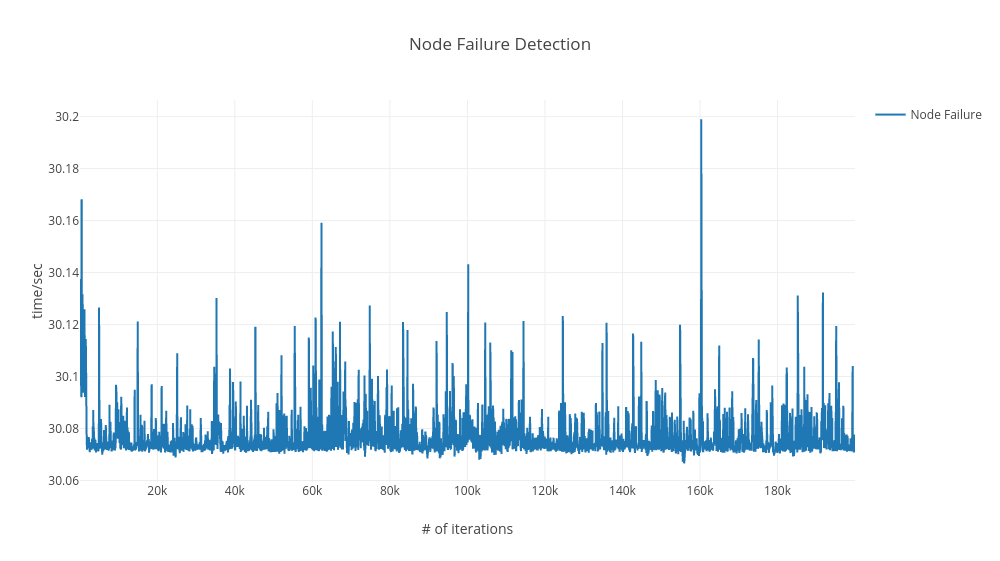
\includegraphics[width=1\textwidth]{figures/benchmark_node.png}
	\caption{Node Failure Detection}
	\label{fig:benchmark_node}
\end{figure}

\subsection{Link Failure}

The purpose of this benchmark is to find the time taken to detect a channel link failure in the topology. Channel link failure is here meant to be physical link failure. If any of the channel links between the nodes that are running the provenance API daemon and pipeline daemon are failed then messages sent via this nodes will be failed to reach the other nodes.

We need to measure the time taken metric for our provenance system to detect such a failure. In our provenance database, heartbeat messages are sent by each node are stored in the HEARTBEAT table. Also to check if the neighbouring nodes are active and also to detect link failures, we also send messages to neighbours and each node will transmit those messages to the provenance database. 

So the main tables that are needed to perform this benchmark are,
    \begin{itemize}
        \item Node
        \item HeartBeat
    \end{itemize}

\subsubsection{Method to generate a link failure}

There are two ways to generate a link failure,
    \begin{itemize}
        \item During the deployment of the topology, 'host\_next' parameter in the topology yaml file which is used to provide a virtual link between containers(nodes). We will be changing the name of this field to some random value and thus making the two containers unreachable. There-by simulating a link failure between nodes in the provenance system.
        \item Another method to simulate a link failure is to kill one container(node) itself. Because once the deployment is done and the topology is running in the provenance system, killing the container(node) is the only way to simulate the link failure in the docker environment.
    \end{itemize}

Here we have used the first method and during the deployment itself we provide a wrong connection between the nodes and we run the benchmark test to detect those failures.

\subsubsection{Logic used to detect link failure}

We will be querying the Node table to get the list of successor for each node. Once we got the successor for a particular node, then we query the heartbeat table to get the rows with the id of the successor node and also with its own id.

Once we get the rows, if heartbeat rows are available for the node and its neighbour then we can be sure that both the nodes are active.
The next check we need to perform is to find if the channel field in the heartbeat table row with the successor id contains the node id.
If the node id is present then we can conclude that channel link is also active. We also need to perform an additional check to find out if the channel field is less than 30 seconds old. Because each node will be sending the heartbeat messages every 30 seconds and we need to be sure that the channel is active currently.

\subsubsection{Result}

Following graph has been generated from the results obtained,

\begin{figure}[H]
	\center
	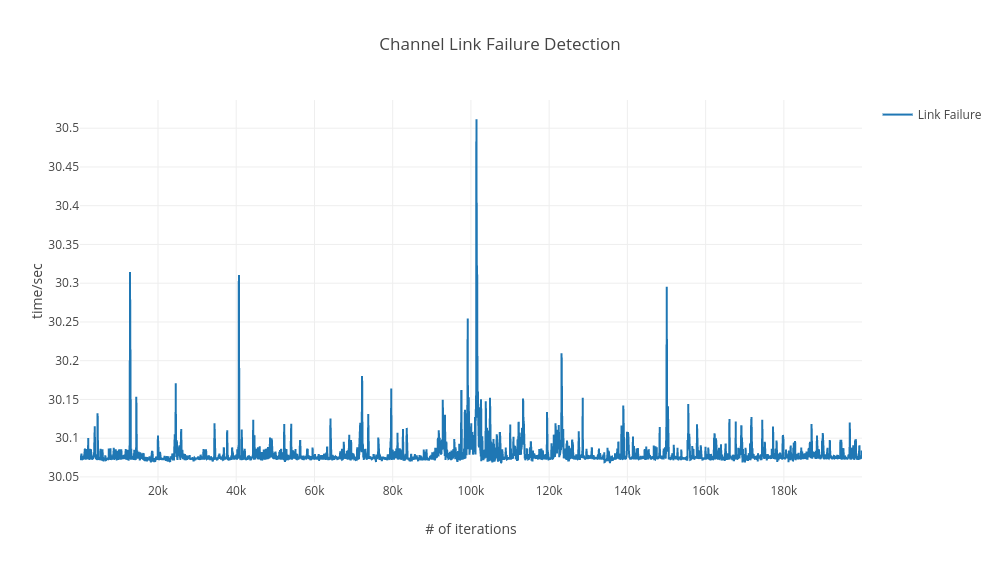
\includegraphics[width=1\textwidth]{figures/benchmark_link.png}
	\caption{Link Failure Detection}
	\label{fig:benchmark_link}
\end{figure}

\subsection{Pipeline Failure}

The purpose of this benchmark is to find the time taken to detect a pipeline daemon failure in the topology. Pipeline daemon failure is here meant to be process failure in a node that is running the pipeline API. If the process in a node that is running the pipeline API daemon are failed then heartbeat messages and provenance messages will not be processed in this node and sent to the database and also not sent to the neighbouring nodes in the topology.

We need to measure the time taken metric for our provenance system to detect such a failure. In our provenance database, heartbeat messages are sent by each node from the pipeline daemon and are stored in the HEARTBEAT table.

So the main tables that are needed to perform this benchmark are,
    \begin{itemize}
        \item Node
        \item HeartBeat
    \end{itemize}

\subsubsection{Method to generate a pipeline daemon failure}

Method to simulate a pipeline daemon failure is to kill the container(node) itself. This is similar to the Node failure detection benchmark we have done earlier. Here the workload generator will introduce failures continuously at regular intervals by killing the docker container and restarting the docker container. This killing and restarting process will happen throughout the benchmark.

\subsubsection{Logic used to detect pipeline daemon failure}

We will be querying the NODE table to get the list of nodes that are running the pipeline daemon. Once we got the node id for a particular node, then we query the heartbeat table to get the rows with that id. 
Once we get the rows, if heartbeat rows are available for the node then we can be sure that the pipeline daemon is active. We also need to perform an additional check to find out if the timestamp field is less than 30 seconds old. Because each pipeline daemon will be sending the heartbeat messages every 30 seconds and we need to be sure that the pipeline daemon is active currently. We will store the timestamp value each time in the benchmark and compare it next time with the previous value to find out if the heartbeat message is the latest one.

\subsubsection{Result}

Following graph has been generated from the results obtained,

\begin{figure}[H]
	\center
	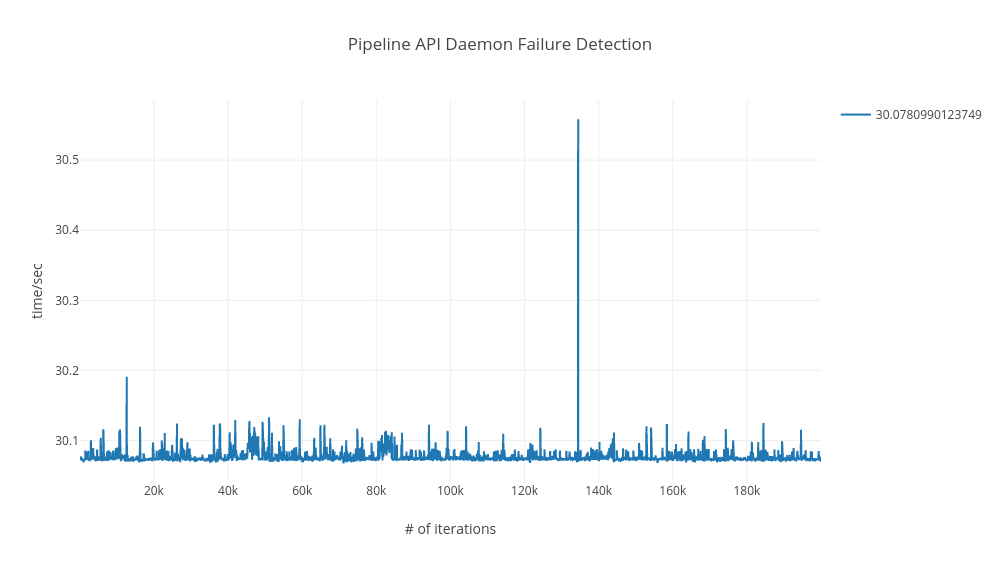
\includegraphics[width=1\textwidth]{figures/benchmark_pipeline.png}
	\caption{Pipeline API Daemon Failure Detection}
	\label{fig:benchmark_pipeline}
\end{figure}

\subsection{Provenance Daemon Failure}

The purpose of this benchmark is to find the time taken to detect a provenance daemon failure in the topology. Provenance daemon failure is here meant to be process failure in a node that is running the provenance API. If the process in a node that is running the provenance API daemon are failed then provenance data will not be processed in this node and sent to the database.

We need to measure the time taken metric for our provenance system to detect such a failure. In our provenance database, provenance data are sent by each node are stored in the PROVENANCETABLE table.

So the main tables that are needed to perform this benchmark are,
    \begin{itemize}
        \item Node
        \item Provenancetable
    \end{itemize}

\subsubsection{Method to generate a provenance daemon failure}

Once the deployment is done and docker containers are started, workload generator need to run within each node to kill the process. But that will make the same node to always fail the same provenance daemon. Even if the workload generator script is started in all the nodes then all the provenance daemons will fail at the same time. Coordination between workload generators will generate extra load on the provenance system which will not give the exact results. Hence the workload generator here will directly delete the rows from the PROVENANCETABLE table for half of the nodes in the topology. Thus we generate the provenance daemon failure at regular intervals this way while running the benchmark.

\subsubsection{Logic used to detect provenance daemon failure}

We will be querying the Node table to get the list of nodes. Once we got the node id for a particular node, then we query the PROVENANCETABLE table to get the rows with that id. Initially we will mark the provenance daemon active if we found rows greater than 0 and then we will query the PROVENANCETABLE every 10 seconds delay and again check the count. Previous counts will be stored throughout the benchmark. Provenance Daemon will be marked as active if the count has been increased compared to the previous count value. If the count remains unchanged then Provenance daemon will be marked as failed.

\subsubsection{Result}

Following graph has been generated from the results obtained,

\begin{figure}[H]
	\center
	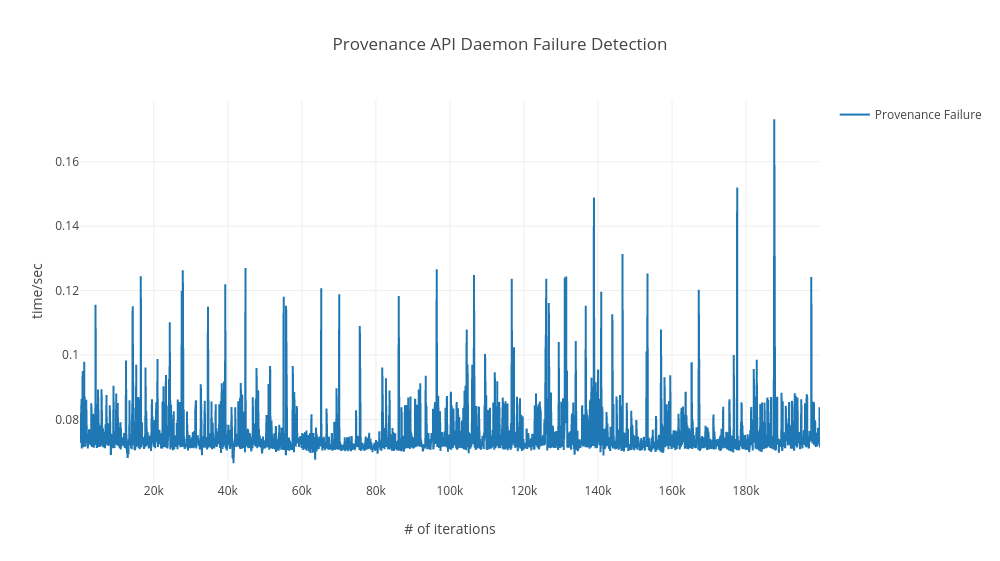
\includegraphics[width=1\textwidth]{figures/benchmark_provenance.png}
	\caption{Provenance API Daemon Failure Detection}
	\label{fig:benchmark_provenance}
\end{figure}


\subsection{Steps to run the failure detection benchmark}


Pull the Benchmark repository from the following link,
https://github.com/Krymnos/idp-benchmark/blob/master/benchmark/

Deploy the complete stack in AWS (deployment steps are explained in the deployment chapter). Once the deployment is done, get the public IP address of the Manager node and this IP address will be used to connect to the cassandra database deployed in our stack. Cassandra IP address will be passed as an external parameter to our failure detection benchmark script.

Run the benchmark script like below(replace the IP address accordingly),

\begin{center}
    python startBenchmark.py -i 18.197.129.37
\end{center}

This script will automatically run all the four failure detection benchmarks and save the output in a folder named "results".


